\documentclass{beamer}

%\usetheme{AnnArbor}
\usetheme{Warsaw}
\usecolortheme{seahorse}
\usecolortheme{rose}
\usefonttheme[onlylarge]{structuresmallcapsserif}
\usefonttheme[onlysmall]{structurebold}
\setbeamerfont{title}{shape=\itshape,family=\rmfamily}
%\setbeamercolor{title}{fg=red!80!black}


%\usecolortheme{wolverine}
\usepackage[utf8]{inputenc}
\usepackage[T1]{fontenc}
\usepackage[french]{babel}
\usepackage{tikz}
\usepackage{animate}
%\usepackage{graphicx}
\usepackage{blkarray}
\usepackage{graphicx}

\title{TRON GAME}
\author[A. Catherine ATTY \\  Sékou DOUMBOUYA \\ Manne Emile KITSOUKOU \\ Amirath Fara OROU-GUIDOU]{A. Catherine ATTY \\  Sékou DOUMBOUYA \\ Manne Emile KITSOUKOU \\ Amirath Fara OROU-GUIDOU}
\institute[Université de Caen Normandie]{Université de Caen Normandie}
\date{\today}
\logo{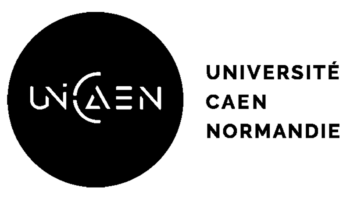
\includegraphics[width=0.2\textwidth]{Images/universite-de-caen-normandie-1-350x0-c-default.png}}

\setbeamertemplate{footline}[frame number]

\begin{document}
    \frame{\titlepage}
    \begin{frame}{Plan}
        \tableofcontents
    \end{frame}


    \section{Introduction}

    \subsection*{Historique du jeu}
    \begin{frame}{Historique du jeu}
        \begin{columns}
            \column{0.6\textwidth}
            \begin{center}
                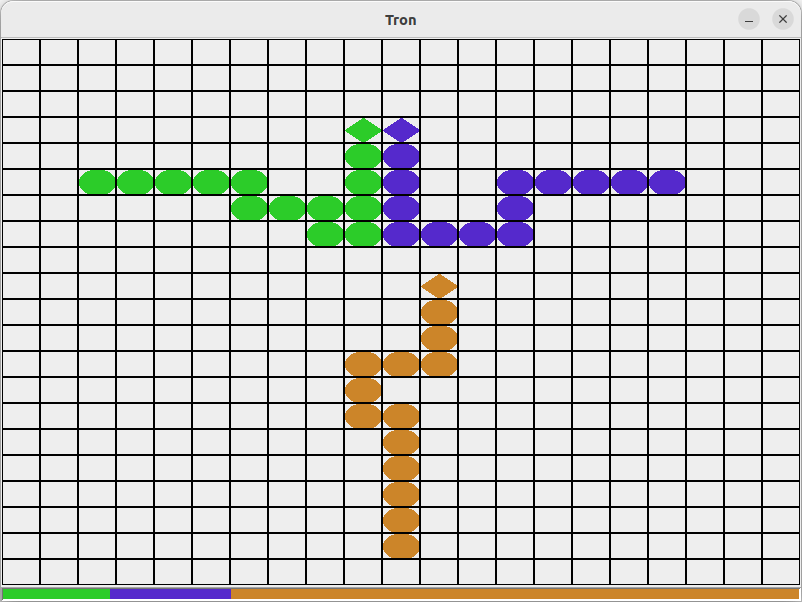
\includegraphics[width=\textwidth]{Images/jeu-tron}
            \end{center}
            \column{0.4\textwidth}
            \begin{block}{Qu'est ce que le jeu TRON ?}
                \pause
                \begin{itemize}
                    [<+->]
                    \item Jeu d'arcade classique popularisé dans les années 80
                    \item Similaire au jeu du serpent( Snake )
                    \item Le but est d'êtres le dernier joueur en vie
                \end{itemize}
            \end{block}

        \end{columns}
    \end{frame}

    \subsection*{Pourquoi ce projet ?}
    \begin{frame}{Choix du projet}
        \begin{block}{Pourquoi ce projet ?}
            \pause
            \begin{itemize}
                [<+->]
                \item Opportunité d'améliorer ses compétences en programmation et algorithmique
                \item Bonne occasion de découvrir, approfondir et mettre en pratique les algorithmes de recherche adversarial
                \item Curiosité de répondre à la question scientifique
            \end{itemize}
        \end{block}
    \end{frame}


    \section{Problématique}
    \subsection*{État de l'art}
    \begin{frame}{État de l'art}
        \begin{block}{Théorie de Jeu et Recherche Adversarial}
            \pause
            \begin{itemize}
                [<+->]
                \item \alert{Théorie de Jeu}: branche de la mathématique se consacrant à l'étude des situations de jeu dans lesquelles les choix des joueurs sont interdépendants
                \item \alert{Recherche Adversarial}: ensemble des algorithmes permettant de résoudre des problèmes de jeu à somme nulle
                \item \alert{Somme nulle}: le gain d'un joueur est égal à la perte des autres joueurs
            \end{itemize}
        \end{block}
    \end{frame}
    \subsection*{Problème à résoudre}
    \begin{frame}{Problème à résoudre}
        \begin{block}{Que cherchons-nous à résoudre ?}
            \pause
            Quelles sont les déterminants de la performance d'un joueur contre une coalition d'adversaires?\pause
        \end{block}
        \begin{block}{Les déterminants principaux:}
            \begin{itemize}
                [<+->]
                \item La taille de la grille
                \item La profondeur de raisonnement
                \item La taille de la coalition
            \end{itemize}
        \end{block}
    \end{frame}

    \subsection*{Méthodologie}
    \begin{frame}{Méthodologie}
        \begin{block}{Comment cherchons-nous à résoudre le problème ?}
            \begin{itemize}
                \item Mesure et Comparaison de l'efficacité des algorithmes de recherche adversarial
                \item Détermination de l'heuristique et/ou de la combinaison d'heuristiques optimale
                \item Relation entre les déterminants et la performance d'un joueur
            \end{itemize}
        \end{block}
    \end{frame}


    \section{Objectifs}
    \subsection*{Objectifs généraux}
    \begin{frame}{Objectifs généraux}
        \begin{block}{Ce qui doit être fait}
            \begin{itemize}
                \item Dévelopement du jeu TRON
                \item Implémentation des algorithmes de recherche adversarial
                \item Réalisation d'une interface graphique propre et intuitive
                \item Expérimentations et analyses des résultats
            \end{itemize}
        \end{block}
    \end{frame}
    \subsection*{Objectifs additionnels}
    \begin{frame}{Objectifs additionnels}
        \begin{block}{En plus}
            \begin{itemize}
                \item Intégration des heuristiques
                \item Extension du jeu et des algorithmes à la version des coalitions
            \end{itemize}
        \end{block}
    \end{frame}


    \section{Répartition des tâches}
    \begin{frame}{Répartition des tâches}
        \begin{block}{Qui fait quoi ?}
            \begin{itemize}
                \item Amirath Fara OROU-GUIDOU: Implémentation des algorithmes de recherche adversarial
                \item A. Catherine ATTY: Implémentation des algorithmes de recherche adversarial et mise en oeuvre des tests
                \item Manne Emile KITSOUKOU: Développement du model et des heuristiques
                \item Sékou DOUMBOUYA: Réalisation de l'interface graphique
            \end{itemize}
        \end{block}
    \end{frame}


    \section{État d'avancement}
    \begin{frame}{Où en sommes-nous ?}
        \begin{center}
            \begin{figure}
                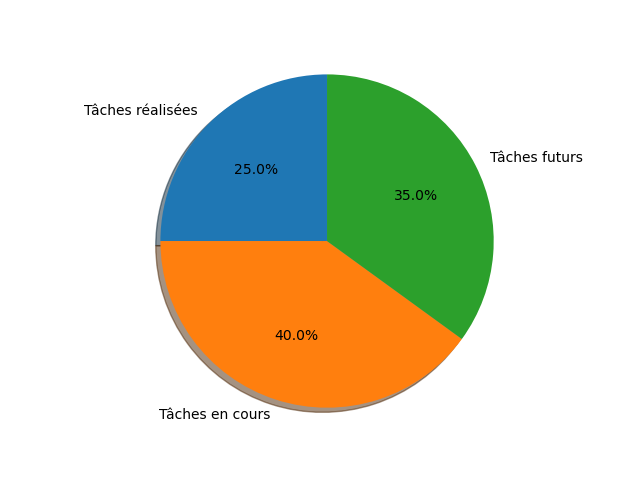
\includegraphics[width=0.7\textwidth]{Images/etat-avancement}
                \caption{État d'avancement}
            \end{figure}
        \end{center}
    \end{frame}
    \subsection*{Tâches réalisées}
    \begin{frame}{Tâches réalisées}
        \begin{block}{Ce qui a été fait}
            \begin{itemize}
                \item Modélisation du jeu
                \item Première approche de l'interface graphique
                \item Implémentation de MaxN, Paranoid
                \item Intégration des heuristiques (Voronoï, GALASP, OpenSpace)
            \end{itemize}
        \end{block}
    \end{frame}
    \subsection*{Tâches en cours}
    \begin{frame}{Tâches en cours}
        \begin{block}{Les tâches en cours de développement}
            \begin{itemize}
                \item Optimisation des algorithmes de recherche adversarial
                \item Amélioration de l'interface graphique
                \item Mise en oeuvre des tests
                \item Extension du jeu et des algorithmes à la version des coalitions
            \end{itemize}
        \end{block}
    \end{frame}
    \subsection*{Tâches à réaliser}
    \begin{frame}{Tâches à réaliser}
        \begin{block}{Les tâches à réaliser}
            \begin{itemize}
                \item Réalisation des expérimentations
                \item Analyse des résultats
                \item Rédaction du rapport
                \item Présentation du projet
            \end{itemize}
        \end{block}
    \end{frame}
    \subsection*{En résumé}
    \begin{frame}
        \begin{center}
            \begin{figure}
                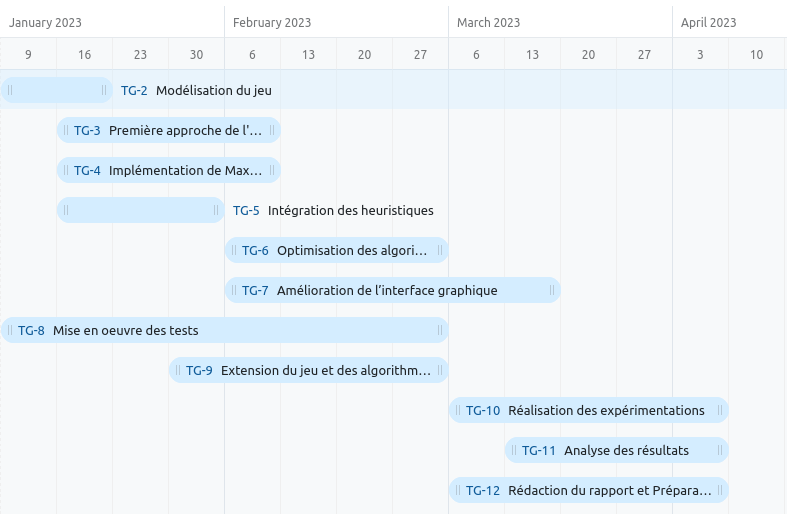
\includegraphics[width=0.8\textwidth]{Images/gant}
                \caption{Gantt des tâches}
            \end{figure}
        \end{center}
    \end{frame}


    \section{Conclusion}
    \begin{frame}{Conclusion}
        \begin{block}{Ce qu'il faut retenir}
            \pause
            \begin{itemize}
                [<+->]
                \item Développement significatif du projet d'étude
                \item Réussite dans les tâches les plus simples du projet
                \item Abord des aspects plus complexes de l'étude
                \item Concentration sur les expérimentations et les analyses dans un futur proche
                \item Objectifs scientifiques et pratiques en ligne de mire
            \end{itemize}
        \end{block}
    \end{frame}

\end{document}
